\documentclass{beamer}
% \usepackage{animate}
\usepackage{multimedia}
\usepackage[english,russian]{babel}

\usepackage{pgfpages}
\setbeameroption{show notes on second screen}
%https://tug.ctan.org/macros/latex/contrib/beamer/doc/beameruserguide.pdf

\usepackage[T2A]{fontenc}
\usepackage[utf8]{inputenc}

\setbeamertemplate{caption}[numbered]

\usetheme{CambridgeUS}
\usecolortheme{dolphin}


\title[Построение изображений]{Процесс построения изображения}
\author[Быковских Д.А.]{Быковских Дмитрий Александрович}
\date{19.09.2026}

\begin{document}
\begin{frame}
	\titlepage
\end{frame}

\begin{frame}{Содержание}
	\begin{itemize}
		\item
		Структура 3D-сцены
		\item
		Графический стек приложения
		\item
		Распределение вычислений
		\item
		Модель графического конвейера
		\item
		Характеристики видеокарты
	\end{itemize}
\end{frame}

\section{Процесс построения изображения}

\begin{frame}{Из скольких объектов состоит сцена?}
	\begin{figure}
		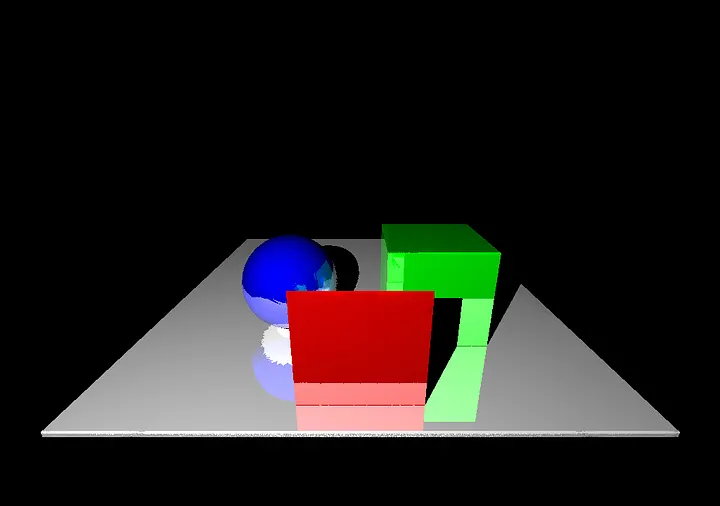
\includegraphics[width=0.75\textwidth]{images/simple_3d_scene.png}
		\caption{Простая 3D-сцена}
	\end{figure}
	\note{
		{
			\usebeamercolor[bg]{note page}%
			Сцена состоит из четырёх видимых объектов и двух невидимых объектов.
			Два невидимых объекта --- камера и источник света.
		}
	}
\end{frame}

\begin{frame}{Рендеринг сцены}
	\begin{figure}
		\href{https://studio.blender.org/training/blender-fundamentals-45-lts/blender_4-5_lts_render-settings/}{
		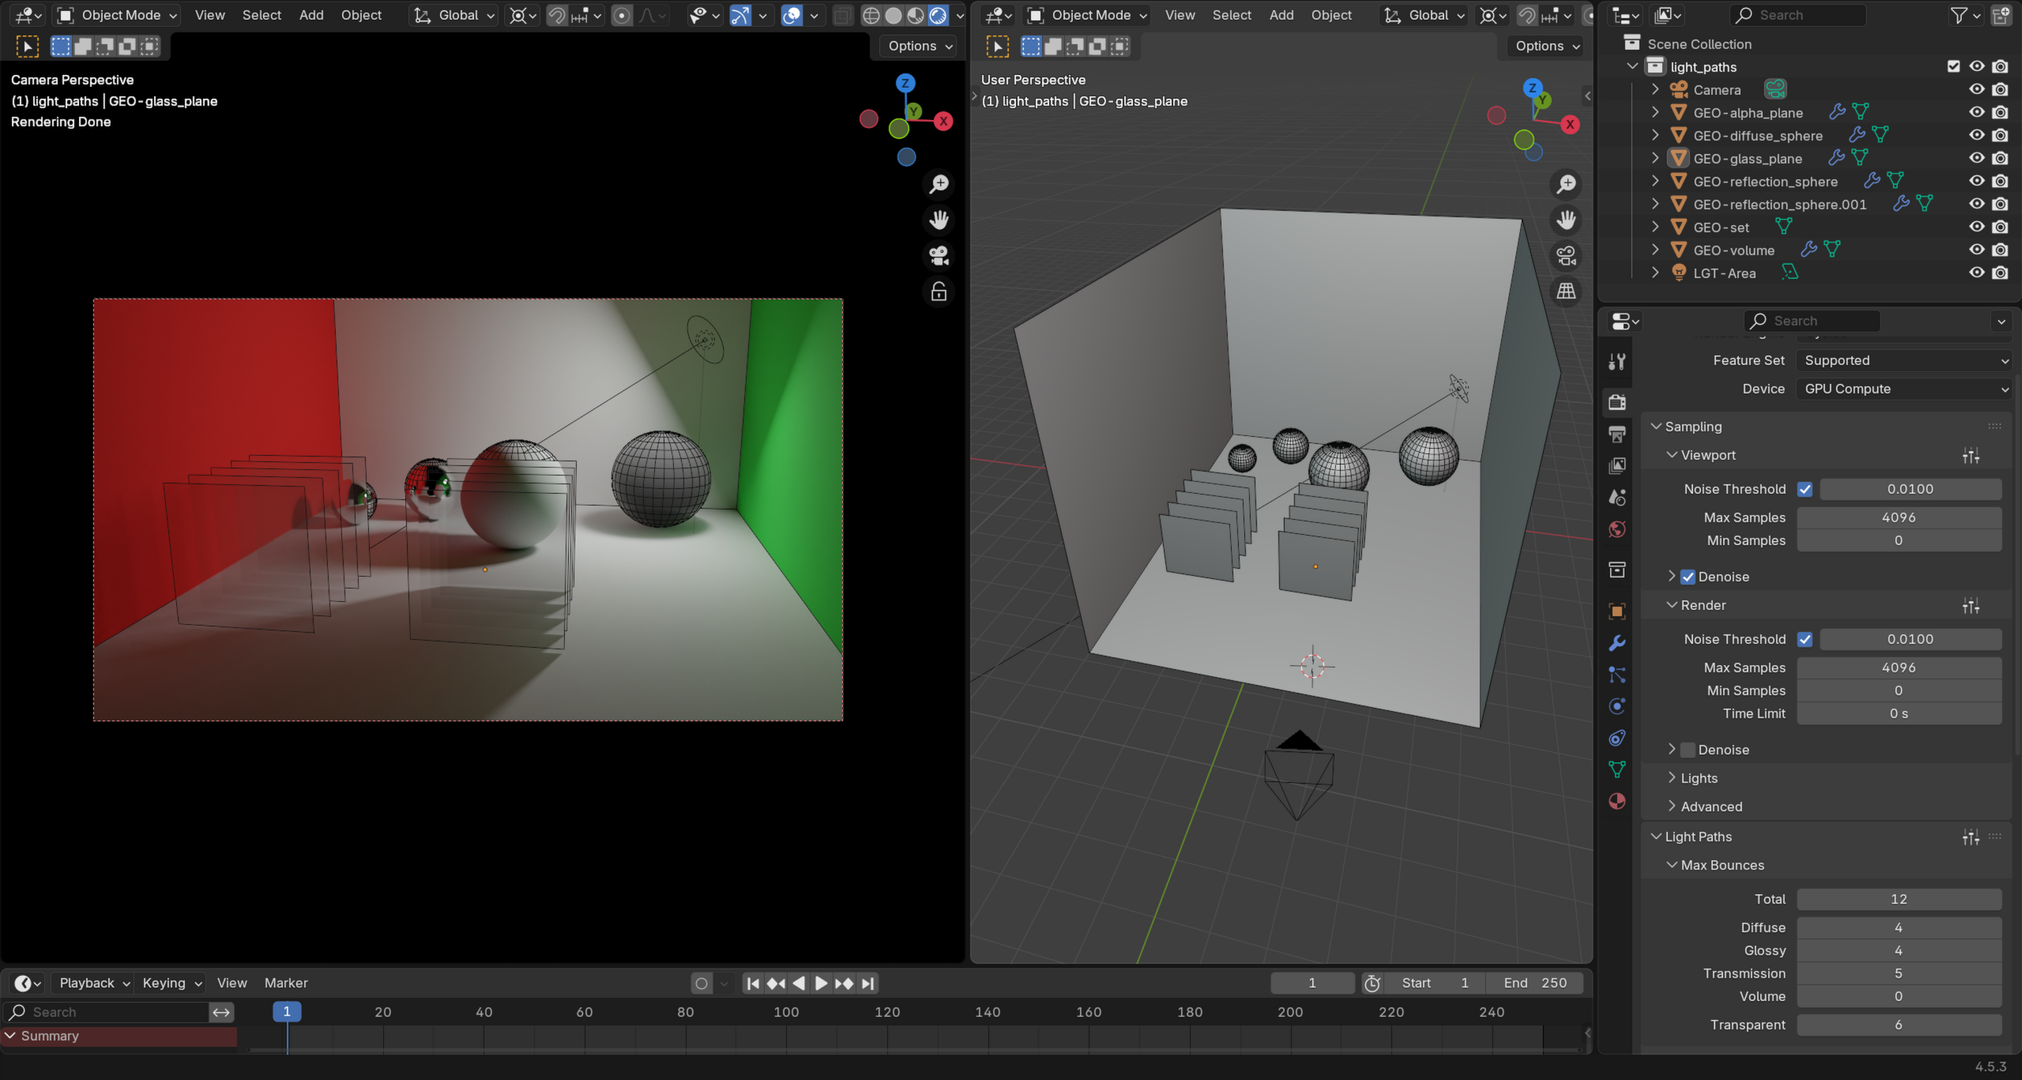
\includegraphics[width=0.95\textwidth]{images/scene_rendering.png}}
		\caption{Рендеринг сцены в blender}
	\end{figure}
	
	\note{
		Структура 3D-сцены:
		\begin{itemize}
			\item Объекты -> Полигоны -> Вершины -> Атрибуты
			\item Источники света -> Атрибуты
			\item Камера -> Атрибуты
		\end{itemize}
	}
\end{frame}

\section{Графический стек приложения}

\begin{frame}{Многоуровневая модель графического стека приложения}
	\begin{figure}
		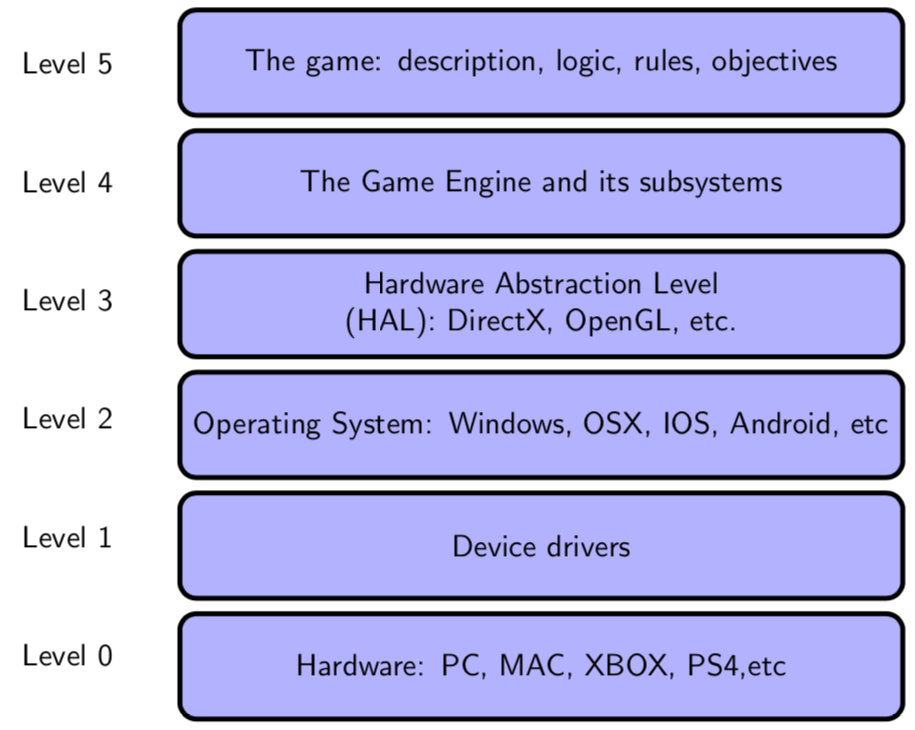
\includegraphics[width=0.65\textwidth]{images/Game_architecture.png}
		\caption{Структура графического стека приложения}
	\end{figure}
	
	\note{
		\textbf{Терминология}
			{\scriptsize
			
			\textbf{Драйвер (видеодрайвер)} --- системный модуль, управляющий конкретным GPU и реализующий графический API в данной ОС.

			\textbf{Спецификация} --- формальное описание графического API: функции, типы, состояния и гарантии поведения реализации (OpenGL, Vulkan). Это документ, а не исполняемый код.

			\textbf{Графический API} --- программный интерфейс, через который приложение отдаёт работу GPU (контекст, буферы, текстуры, шейдеры, вызовы отрисовки).

			\textbf{Графическая библиотека} --- реализация спецификации (Mesa) либо тонкая обёртка над API: загрузка функций, создание контекста, математика, загрузка изображений и моделей.

			\textbf{Графический фреймворк} --- каркас приложения: задаёт архитектуру и цикл работы, вызывает код пользователя (инверсия управления). Выше библиотеки, без готовых игровых подсистем (физика, ИИ, сеть).

			\textbf{Графический движок} --- подсистема визуализации: сцена, материалы, освещение, отправка команд в API.

			\textbf{Игровой движок} --- надстройка над API/библиотекой: графический движок плюс физика, анимация, аудио, I/O, скрипты; часто сеть.

			\textbf{Графические редакторы} --- программы для создания и правки ассетов (растр, вектор, 3D, воксели).

			~
		}
	}
	
\end{frame}

\begin{frame}{API (Application Programming Interface) и графические библиотеки}

	{\small
		\textbf{OpenGL (1992, Silicon Graphics Inc.)} \\
		Открытая кроссплатформенная спецификация для работы с 2D- и 3D-графикой

		\textbf{Mesa (1995, Brian Paul)} \\
		Свободная реализация графических API: OpenGL (позже Vulkan и др.) с открытым исходным кодом

		\textbf{DirectX (1995, Microsoft)} \\
		Пакет API для разработки игр и мультимедийных приложений на платформе Windows

		\textbf{WebGL (2011, Khronos Group)} \\
		Графический API для веб-браузеров

		\textbf{Mantle (2013, AMD)} \\
		Спецификация низкоуровневого API

		\textbf{Vulkan (2016, Khronos Group)} \\
		Низкоуровневый (требует явного управления памятью и ресурсами), высокопроизводительный кроссплатформенный графический API
	}

	\note{
		\textbf{Пример взаимодействия спецификации, API и библиотек}
		\begin{enumerate}
			\item Спецификация OpenGL~4.5 описывает контракт:
			
			\texttt{DrawArrays(TRIANGLE\_FAN, first, count)} строит примитивы из VAO.
			
			\item API --- вызов в коде:
			
			\texttt{glDrawArrays(GL\_TRIANGLE\_FAN, 8, 12);}
			
			\item Реализация --- драйвер / Mesa.
		\end{enumerate}
		Библиотеки вокруг API:
		\begin{itemize}
			\item \texttt{glfwCreateWindow} --- где взять framebuffer;
			\item \texttt{glewInit} --- где взять адрес \texttt{glDrawArrays};
			\item \texttt{glm::vec3} --- какие числа положить в VBO.
		\end{itemize}
	}

\end{frame}

\begin{frame}{Mesa}
			\textbf{Mesa} --- открытый проект, который предоставляет реализацию различных графических API (таких как OpenGL, OpenGL ES, Vulkan, OpenCL и др.).

	Mesa поддерживает реализацию OpenGL для устройств, разработанных Intel, AMD, NVIDIA, Qualcomm и др., включая виртуальные графические процессоры VMware и VirGL.
	Также есть несколько программных рендереров: Softpipe (драйвер Gallium) и LLVMpipe (высокоскоростной растеризатор на основе LLVM/JIT).

	\note{
		Проект начал разрабатывать Брайан Пол (Brian Paul) в 1993 году. Основная цель заключалась в реализации API, совместимого с OpenGL, по мотивам IRIS GL.

		Первая версия вышла в 1995 году с разрешения SGI. Название Mesa, по словам Пола, просто пришло в голову; SGI запретила использовать в имени слова <<Open>> и <<GL>>.

		https://docs.mesa3d.org/history.html
		% 	% https://www.mesa3d.org/

	}

\end{frame}

\section{Распределение вычислений}

\begin{frame}{Распределение вычислений между CPU и GPU}{CPU (Central Processing Unit) и GPU (Graphics Processing Unit)}
	%GPU а термин не ввел.
	\begin{figure}
		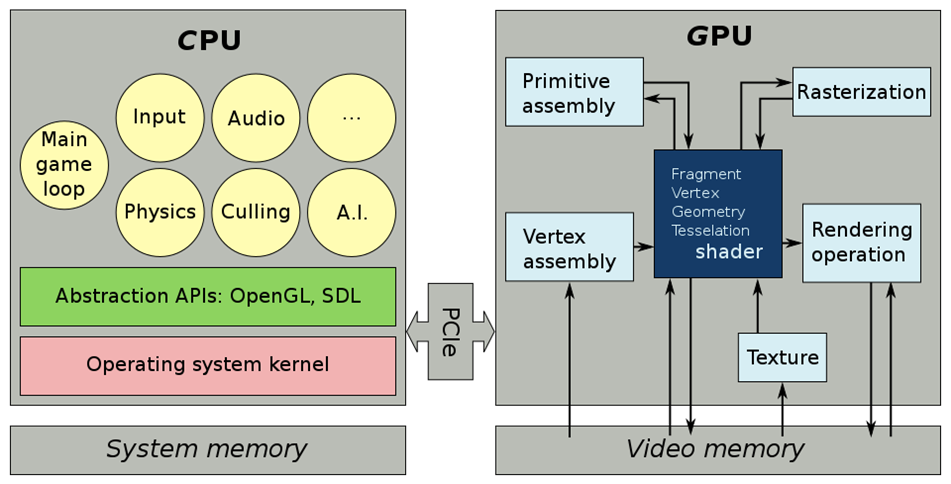
\includegraphics[width=0.95\textwidth]{images/Calculation_distribution_scheme.png}
		\caption{Принципиальная схема распределения вычислений}
	\end{figure}


	\note{
		\begin{figure}
			\href{https://jagatplay.com/2024/03/news/sony-akan-umumkan-ghost-of-tsushima-versi-pc-minggu-ini/}{
				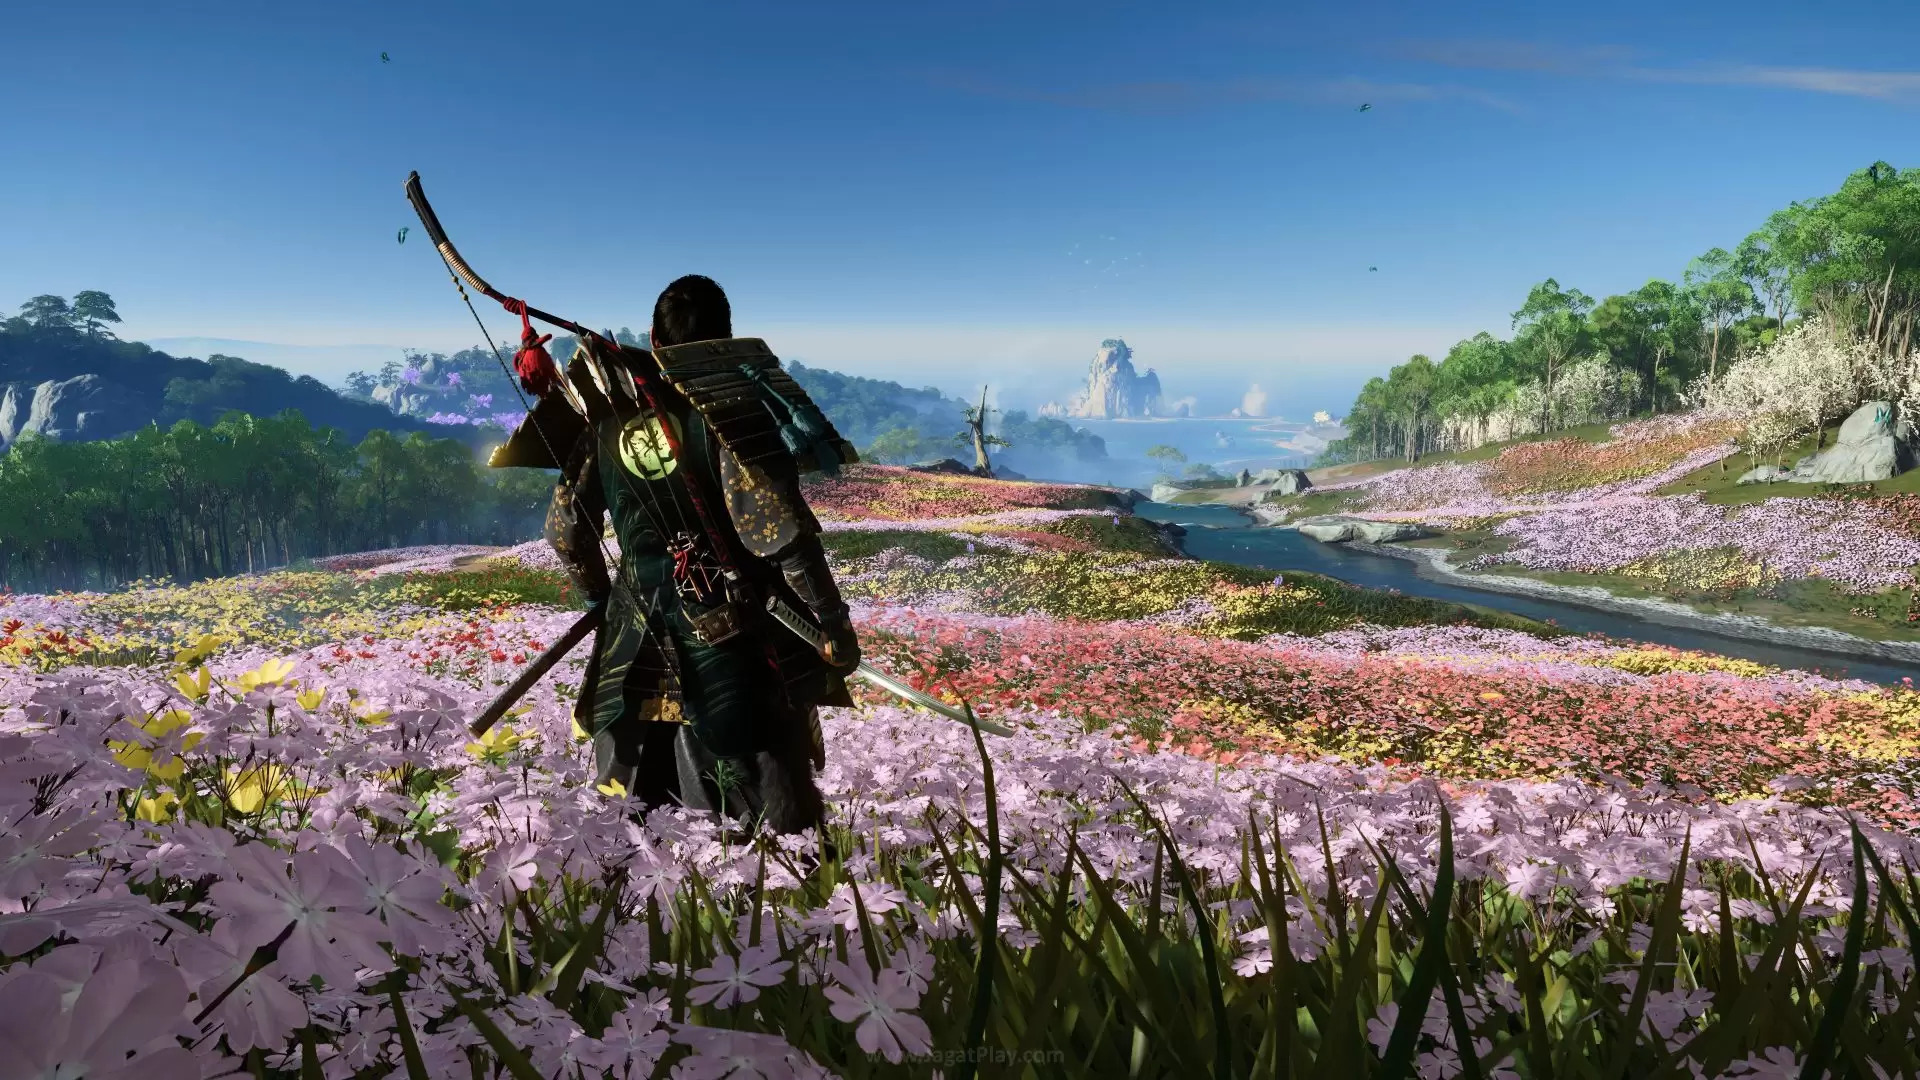
\includegraphics[width=0.9\textwidth]{images/Ghost_of_Tsushima.jpeg}}
			\caption{Ghost of Tsushima (2024, Призрак Цусимы)}
		\end{figure}

	}
\end{frame}

\section{Модель графического конвейера}

\begin{frame}{Упрощённая схема графического конвейера}
	\begin{columns}
		\begin{column}{0.5\textwidth}
			\begin{figure}
				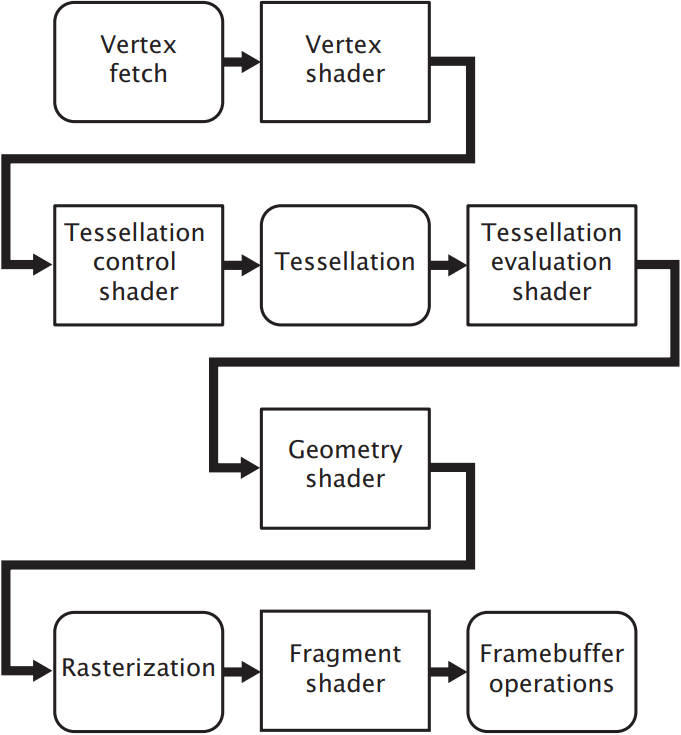
\includegraphics[width=0.9\textwidth]{images/Simplified_model_of_the_graphics_pipeline.png}
				\caption{Порядок вычисления шейдеров}
			\end{figure}
		\end{column}
		\begin{column}{0.5\textwidth}

			{\footnotesize

			Загрузка данных

			{\hfill Вершины (vertices)}

			\textbf{Вершинный шейдер}

			{\hfill Группа вершин (primitives/patches)}

			\textbf{Шейдер управления тесселяцией}

			Тесселяция

			\textbf{Шейдер оценки тесселяции}

			{\hfill Примитивы (primitives)}

			\textbf{Геометрический шейдер}

			{\hfill Примитивы (primitives)}

			Растеризация и интерполяция

			{\hfill Фрагменты (fragments)}

			\textbf{Пиксельный (фрагментный) шейдер}

			{\hfill Фрагменты (fragments)}

			Операции с буфером кадра

			{\hfill Пиксели (pixels)}
			}
		\end{column}
	\end{columns}

	\note{
		\begin{figure}
			\href{https://mshobby.wordpress.com/2013/05/04/tessellation-a-wonder-technology-in-graphics/}{
				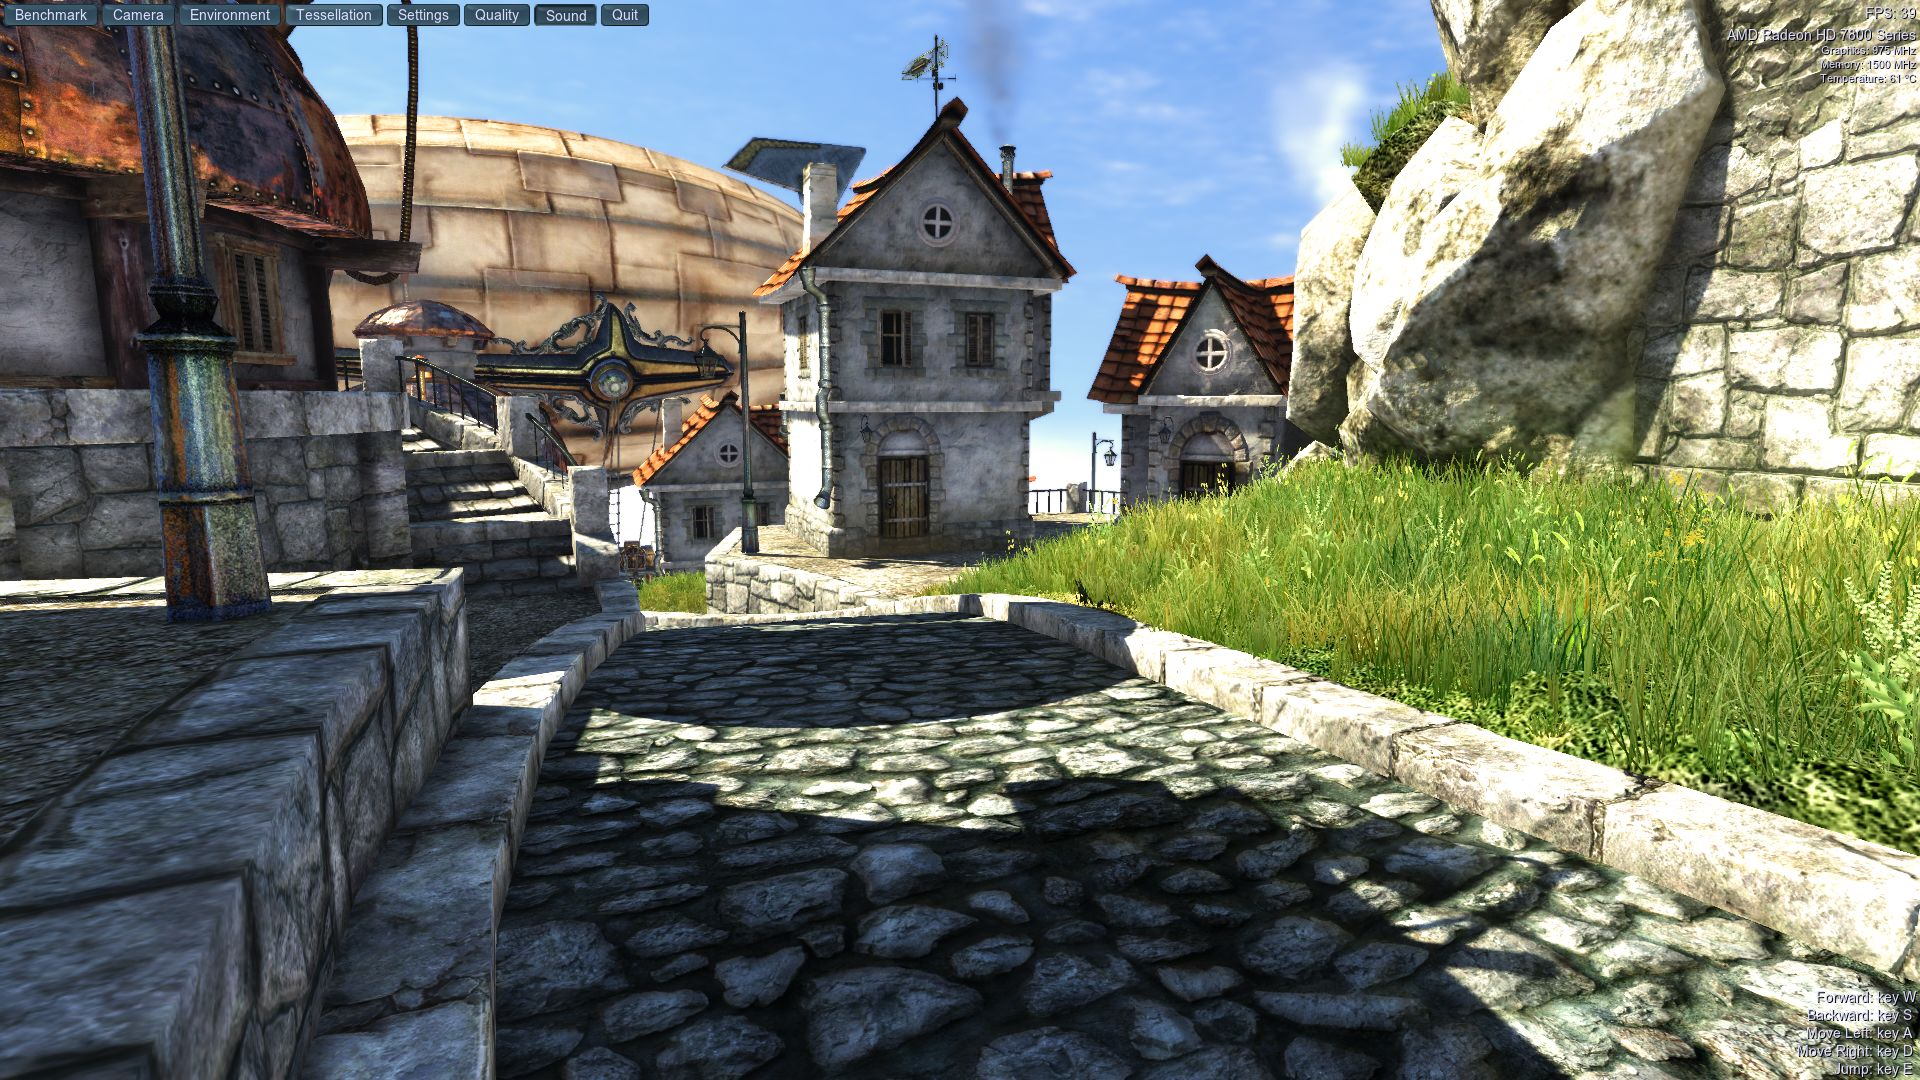
\includegraphics[width=0.47\textwidth]{images/wo_tesselation.jpg}
				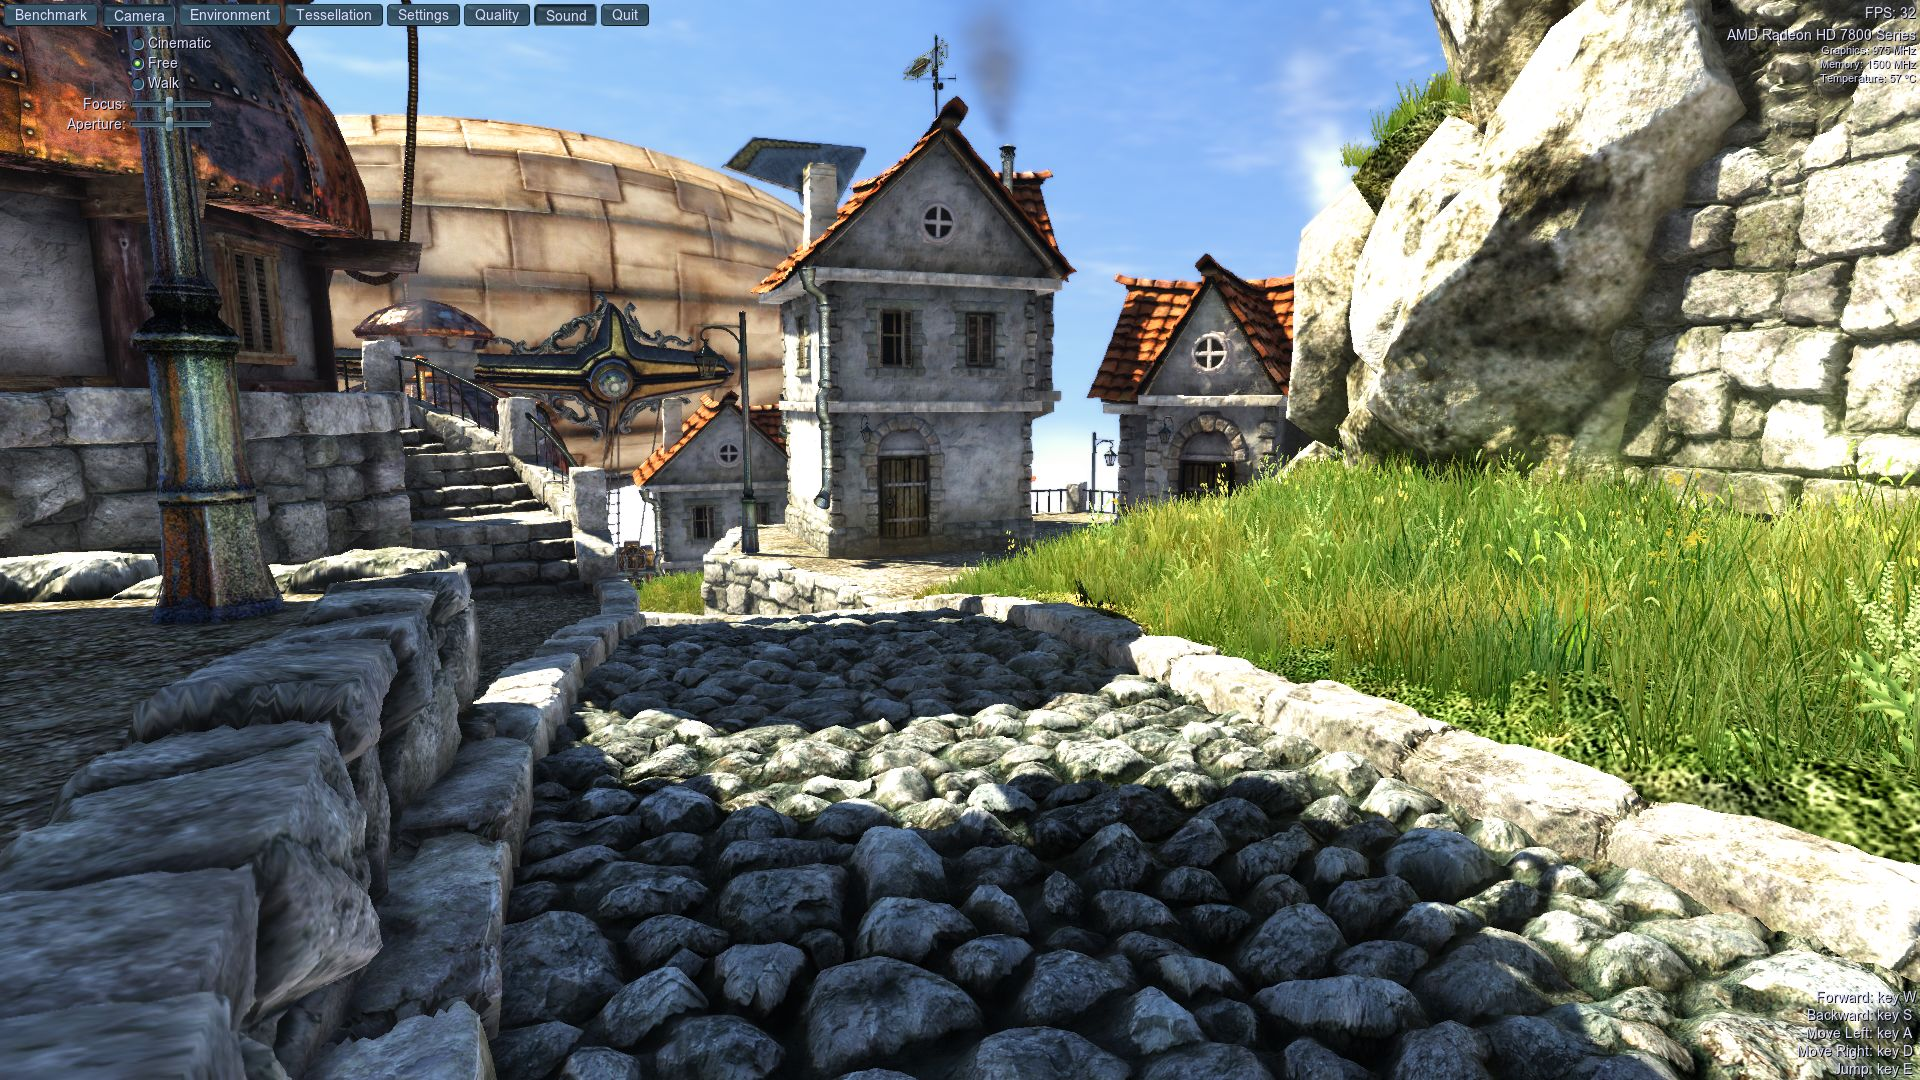
\includegraphics[width=0.47\textwidth]{images/w_tesselation.jpg}
				}
			\caption{
				{\scriptsize
				DirectX 11 (2009): без тесселяции (слева) и с тесселяцией (справа)}}
		\end{figure}


		\vspace{-1em}
		{\footnotesize

			\textbf{Вершинный и пиксельный шейдеры:}
			
			 DirectX 8.0, 2000; OpenGL 2.0, 2004
				
			\textbf{Геометрический шейдер:}
			
			DirectX 10, 2006; OpenGL 3.2, 2009
			
			\textbf{Шейдеры тесселяции:}
			
			DirectX 11, 2009; OpenGL 4.0, 2010
		}
	}

\end{frame}

\begin{frame}{Схема графического конвейера}
	\begin{figure}
		\href{https://www.researchgate.net/figure/Outline-of-the-graphics-pipeline_fig1_281810652}{
			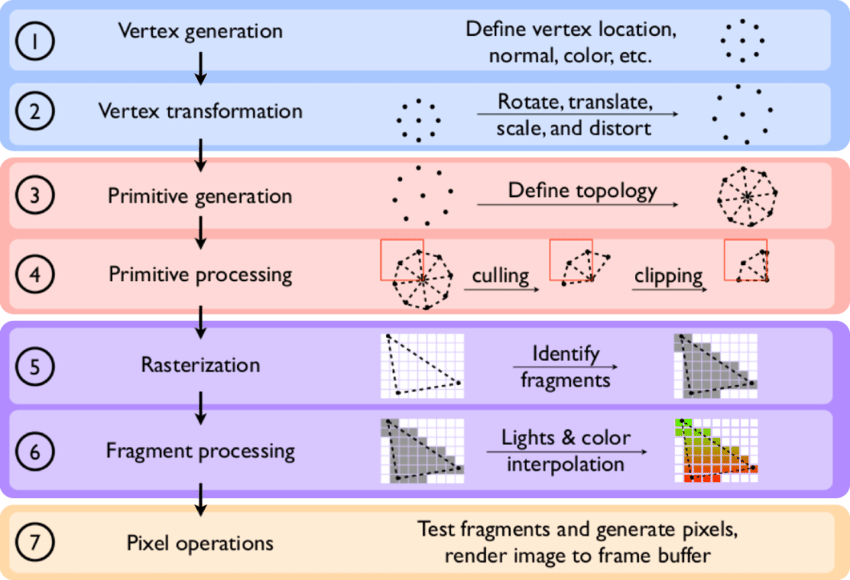
\includegraphics[width=0.75\textwidth]{images/Outline-of-the-graphics-pipeline.png}}
		\caption{Схема графического конвейера}
	\end{figure}
\end{frame}

\begin{frame}{Растеризация (Rasterization)}
	
	\textbf{Растеризация} --- метод рендеринга, который преобразует 3D-сцену в 2D-изображение, отображаемое на экране. 
	Этот метод долгое время является основным подходом в компьютерной графике для создания изображений в реальном времени 
	и отличается высокой производительностью, так как оптимизирован для работы на GPU.

	\begin{figure}
		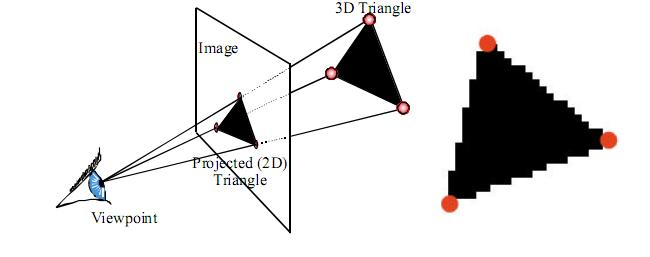
\includegraphics[width=0.75\textwidth]{images/rasterization.jpg}
		\caption{
			\href{https://racketboy.com/retro/about-video-games-rasterization-and-z-buffer}{Схема построения изображения с помощью растеризации}
		}
	\end{figure}

	\note{

		% \href{https://www.etymonline.com/word/raster#etymonline_v_36914}{\textbf{Растр}}
		\textbf{Растр}
		(Raster, 1934) --- сканирующее поле.

		Недостаток растеризации заключается в том, что тени и отражения приходится добавлять отдельными методами.

	}

\end{frame}

\begin{frame}{Конвейер рисования в OpenGL}
	\begin{figure}
		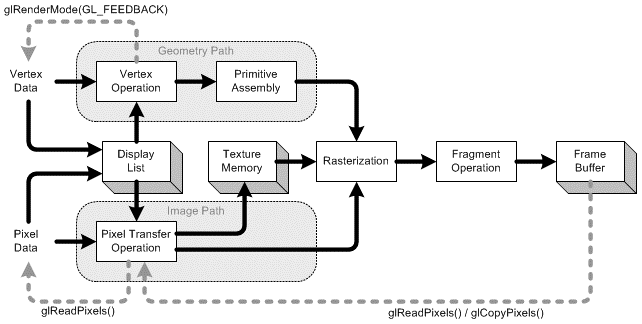
\includegraphics[width=0.95\textwidth]{images/OpenGL_graphics_pipeline.png}
		\caption{Конвейер рисования OpenGL}
	\end{figure}
\end{frame}

\section{Характеристики видеокарты}

\begin{frame}{Характеристики видеокарты}{}

	\begin{columns}
		\begin{column}{0.5\textwidth}
			{\footnotesize

			\textbf{Графический процессор (видеочип)}

			Число транзисторов, млрд.
	
			Техпроцесс, нм
			
			Тактовая частота, ГГц
			
			Количество шейдерных ядер (ALU, Arithmetic Logic Unit)
			
			Тензорные ядра (Tensor Cores, NVIDIA)
		
			RT-ядра (Ray-Tracing Cores, NVIDIA)

			Блоки растровых операций (ROP)

			Блоки наложения текстур (TMU)

			\vspace{1em}

			\textbf{Скорость заполнения (Fill Rate)}
							
			Пиксельная --- ROPs $\times$ частота
				
			Текстурная --- TMUs $\times$ частота

		
			}
		\end{column}
		\begin{column}{0.5\textwidth}
			{\footnotesize

			\textbf{Графическая память}
		
			Разрядность шины, бит
			
			Тип микросхем (GDDR7 SDRAM)
			
			Тактовая частота, ГГц
			
			Объём, Гбайт

			\vspace{1em}

			\textbf{Другие атрибуты}
			
			Размеры
			
			Тип охлаждения
			
			Шина I/O (PCIe)
			
			Мощность, Вт (Энерговыделение)
			
			Производительность шейдерных ALU (FP32/FP64/FP16)

			% \vspace{25mm}

			}
		\end{column}
	\end{columns}

	
	
	
	\note{
	
		Описание самой мощной игровой видеокарты на 2026~г. NVIDIA GeForce RTX 5090

		https://www.techpowerup.com/gpu-specs/geforce-rtx-5090.c4216

		С различными характеристиками можно ознакомиться:

		https://www.thg.ru/graphic/graphic\_card\_faq\_ii/index.html
		
		\tiny
		{\small
		Скорость заполнения (Fill Rate)
		}
	
		С какой скоростью графический процессор может выдавать пиксели.
		Выделяют два типа скорости заполнения: пиксельную (pixel fill rate, ${PFR = ROP \cdot Hz}$) и текстурную (texture fill rate, ${TFR = TMU \cdot Hz}$).

		Исторически (середина 2000-х) ATi и nVidia считали текстурную скорость заполнения по-разному. nVidia умножала число пиксельных конвейеров на тактовую частоту, ATi --- число текстурных блоков на тактовую частоту. Оба способа были корректны для тогдашних архитектур, где у nVidia был один текстурный блок на пиксельный конвейер.

		{\small
		Блоки наложения текстур (Texture Mapping Unit, TMU)
		}

		Текстуры следует выбрать и отфильтровать. Эта работа выполняется блоками наложения текстур, которые работают совместно с блоками пиксельных и вершинных шейдеров. 
		Работа TMU заключается в применении текстурных операций над пикселями.

		{\small
		Блоки растровых операций (Raster Operations Pipeline, ROP)
		}

		Процессоры растровых операций отвечают за запись пиксельных данных в память. Скорость, с которой выполняется эта операция, является скоростью заполнения (fill rate). 
		Производительность (и число) ROP уже редко используется для оценки скорости видеокарты, т.к. перестала быть узким местом. 

		\_
	}
	
\end{frame}

\begin{frame}{Характеристики видеокарты}{Memory Hierarchy}
	\begin{figure}
		\href{https://www.researchgate.net/profile/M-Clark/publication/51927898/figure/fig4/AS:668607537233921@1536419867027/A-schematic-of-the-memory-hierarchy-of-the-Nvidia-Fermi-architecture-with-the-peak.png}{
			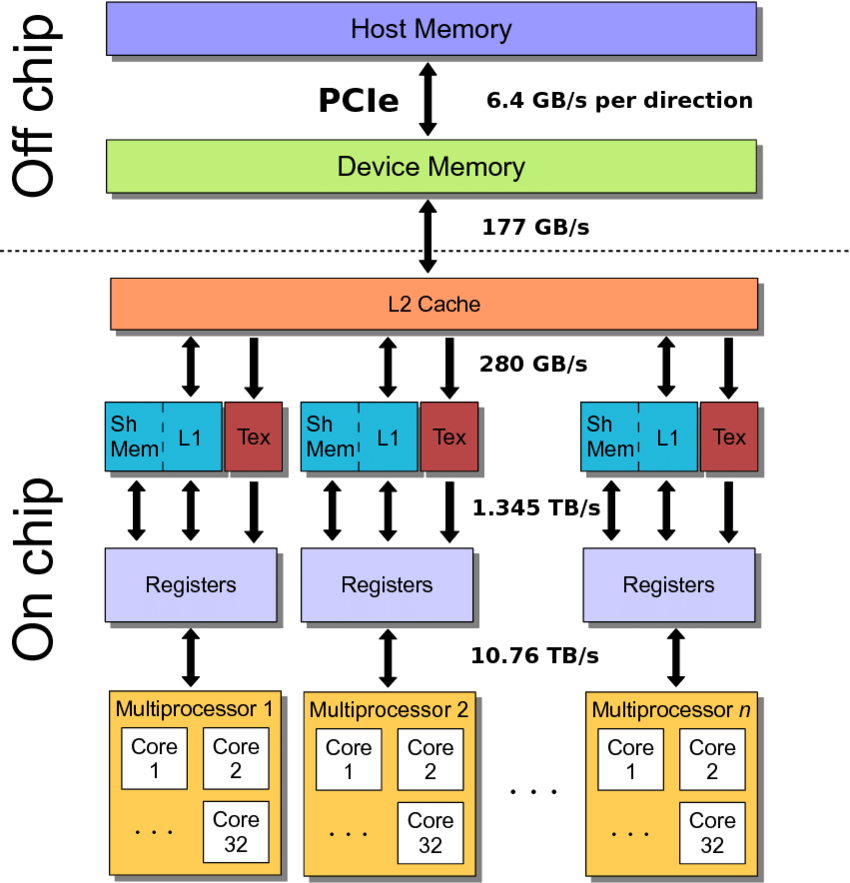
\includegraphics[width=0.45\textwidth]{images/Nvidia_Fermi_architecture_memory.png}}
		\caption {Nvidia Fermi Architecture Memory}
	\end{figure}
	
	\note{
	}
\end{frame}

\end{document}
